\documentclass[11pt]{article}
\usepackage[letterpaper,margin=1in]{geometry}
\usepackage[T1]{fontenc}
\usepackage{lmodern}
\usepackage{microtype}
\usepackage{amsmath,amssymb}
\usepackage{graphicx}
\usepackage{booktabs}
\usepackage[font=small,labelfont=bf]{caption}
\usepackage{xcolor}
\usepackage[colorlinks=true,linkcolor=blue!50!black,citecolor=blue!50!black,urlcolor=blue!50!black]{hyperref}

\newcommand{\Prob}{\mathbb{P}}

\title{Timing of Random Step-Size Perturbations\\ and Uncertainty near the Convergence Boundary}
\author{Arav Rawat}
\date{November 2026}

\begin{document}
\maketitle

\noindent
This note follows up on the earlier report on noise and the fractal convergence boundary of gradient descent for regularized scalar factorization~\cite{liang2026}. As suggested, it addresses one question: \emph{how does the timing of random step-size perturbations affect uncertainty near the deterministic convergence boundary?} Code: \url{https://github.com/lnxv/fractal-convergence-noise} (\texttt{src/timing.py}, \texttt{src/exp\_timing.py}).

\section{Corrected outcome definitions}

The loss and parameters are unchanged: $L(u,v)=\tfrac12(uv-y)^2+\tfrac{\lambda}{2}(u^2+v^2)$ with $y=0.5$, $\lambda=0.2$, $\eta=1$, and minimizers $\pm(m,m)$, $m=\sqrt{y-\lambda}$. For a run with horizon $T$:
\begin{itemize}
  \item \emph{escape}: $|u_t|$ or $|v_t|$ exceeds $10^8$ (or becomes non-finite) for some $t\le T$;
  \item \emph{reaches $\pm(m,m)$}: does not escape and $\|(u_T,v_T)\mp(m,m)\|<r$ with $r=10^{-3}$;
  \item \emph{unresolved}: does not escape and is within $r$ of neither minimizer.
\end{itemize}
The earlier code assigned a surviving run to whichever stationary point it ended closest to, which is a weaker condition than being within a fixed distance of a minimizer. It also set the selection probability to $\tfrac12$ when no run reached either minimizer; such initializations are now marked as unresolved and are not counted as uncertain. Two unit tests check these definitions. In all experiments below the unresolved fraction is exactly zero (every surviving run ends within $10^{-3}$ of a minimizer by $T=200$), so for random step sizes the correction does not change any number. It may matter for the SGD and additive-noise results of the earlier report, under which iterates keep fluctuating; I have not yet rerun those.

From $n$ independent runs per initialization I estimate $\Prob(\text{escape})$ and $p_\pm$. An initialization is \emph{uncertain for escape} if $0.1<\Prob(\text{escape})<0.9$, and \emph{uncertain for selection} if $\Prob(\text{escape})<0.5$, at least one run reached a minimizer, and $0.1<p_+/(p_++p_-)<0.9$.

\section{Experiments}

All experiments use the window $W_1=[2,2.7]\times[-0.3,0.3]$ on a $101\times101$ grid.
\begin{enumerate}
  \item \emph{Initial perturbation}: $(u_0,v_0)+\varepsilon\,\xi$ with $\xi\sim N(0,I_2)$, then deterministic GD; $\varepsilon\in\{0.001,\dots,0.05\}$.
  \item \emph{Noise during an initial segment}: step sizes $\eta_t=\eta(1+\sigma U_t)$, $U_t\sim U(-1,1)$, for the first $K$ updates, then deterministic GD; $K\in\{10,50\}$, $\sigma\in\{0.01,\dots,0.2\}$.
  \item \emph{Persistent noise}: random step sizes for all updates, same $\sigma$.
\end{enumerate}
The baseline uses $T=200$ and $n=64$. To check robustness I repeated experiments 1, 2 ($K=10$) and 3 with a longer horizon ($T=600$, $n=64$) and with more trials ($T=200$, $n=192$), and fitted each scaling law over all levels and again without the smallest and largest level. Since $\varepsilon$ and $\sigma$ are not comparable strengths, I compare scaling trends rather than values at equal amplitude.

\section{Results}

\begin{figure}[!htbp]
  \centering
  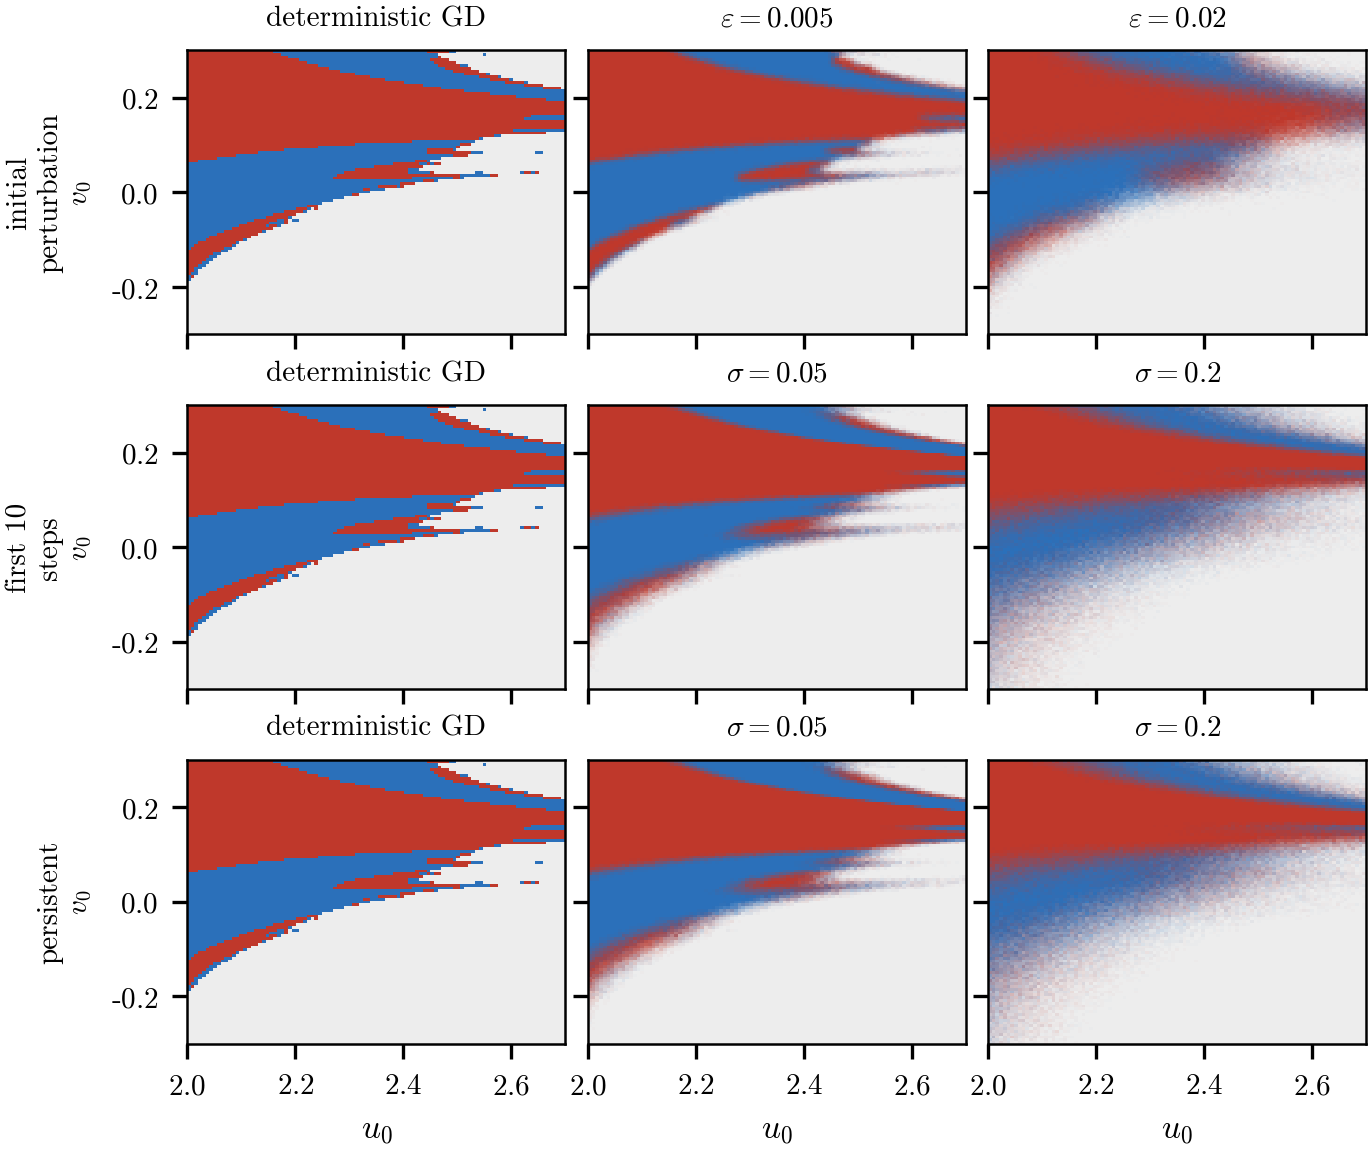
\includegraphics[width=0.8\linewidth]{fig_timing_maps.png}
  \caption{Outcome probabilities in $W_1$. Red and blue intensity give the probabilities of reaching $+(m,m)$ and $-(m,m)$, gray the probability of escape. Rows: initial perturbation, random step sizes in the first 10 updates, random step sizes throughout.}
  \label{fig:maps}
\end{figure}

\begin{table}[!htbp]
  \centering
  \caption{Fraction of $W_1$ with uncertain escape (baseline, $T=200$, $n=64$).}
  \label{tab:values}
  \begin{tabular}{lccccc}
    \toprule
    $\sigma$ & 0.01 & 0.02 & 0.05 & 0.1 & 0.2 \\
    \midrule
    first 10 steps & 0.0198 & 0.0346 & 0.0724 & 0.1340 & 0.2526 \\
    first 50 steps & 0.0198 & 0.0349 & 0.0736 & 0.1359 & 0.2496 \\
    persistent     & 0.0201 & 0.0340 & 0.0737 & 0.1337 & 0.2505 \\
    \bottomrule
  \end{tabular}
\end{table}

\paragraph{Noise after the first few updates hardly matters.} Random step sizes applied only in the first 10 updates give the same uncertain fractions as random step sizes applied throughout, to within $0.003$ at every level (Table~\ref{tab:values}, Figure~\ref{fig:scaling}); $K=50$ is indistinguishable from both. The deterministic dynamics explain why: on a $401\times401$ grid in $W_1$, the outcome of deterministic GD is decided early. I recorded the first step at which an iterate either leaves the box $|u|,|v|\le10$ (all such runs later escape) or enters the ball of radius $0.05$ around a minimizer. The median of this step is $5$, $92\%$ of initializations are decided within $10$ steps and all within $50$. Near the minimizers the Hessian eigenvalues are $0.4$ and $0.6$, so for every step size in $[0.8,1.2]$ the linearized update contracts, and late perturbations of the step size cannot change which minimizer is reached.

\paragraph{Initial and step-size perturbations scale differently for escape.} Table~\ref{tab:exponents} lists the exponents $\beta$ in (uncertain fraction) $\propto(\text{perturbation size})^{\beta}$. For escape, the initial perturbation gives $\beta\approx0.78$ and the random step size $\beta\approx0.84$--$0.85$, a difference of about three standard errors that persists in every robustness check. For minimizer selection the two kinds of perturbation agree ($\beta\approx0.64$--$0.67$). For comparison, the uncertainty exponent of deterministic GD in $W_1$ from the earlier report is $0.74\pm0.01$ for escape and $0.72\pm0.01$ for selection.

\begin{figure}[!htbp]
  \centering
  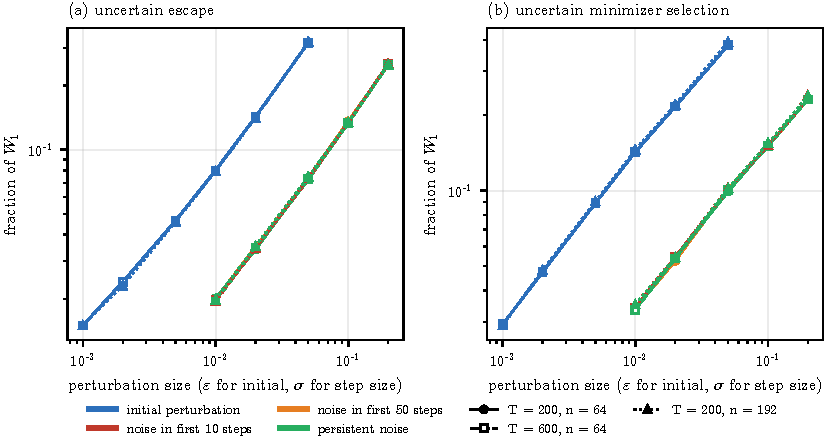
\includegraphics[width=\linewidth]{fig_timing_scaling.pdf}
  \caption{Uncertain fractions in $W_1$ against the perturbation size, on logarithmic axes. Colors: experiments; line styles: baseline and the two robustness runs, which lie on top of each other.}
  \label{fig:scaling}
\end{figure}

\begin{table}[!htbp]
  \centering
  \caption{Fitted exponents $\beta$ (standard error of the fit). ``Narrow'' omits the smallest and largest level. For the initial perturbation and $K=10$, the $T=600$ run reproduces the $T=200$ run exactly, because the dynamics are deterministic after the perturbation and no run is unresolved at $T=200$.}
  \label{tab:exponents}
  \small
  \begin{tabular}{llcccc}
    \toprule
    & & \multicolumn{2}{c}{uncertain escape} & \multicolumn{2}{c}{uncertain selection} \\
    \cmidrule(lr){3-4}\cmidrule(lr){5-6}
    experiment & run & all levels & narrow & all levels & narrow \\
    \midrule
    initial perturbation & $T=200$, $n=64$  & $0.779\,(19)$ & $0.772\,(18)$ & $0.657\,(10)$ & $0.663\,(14)$ \\
                         & $T=200$, $n=192$ & $0.784\,(22)$ & $0.786\,(12)$ & $0.665\,(12)$ & $0.664\,(15)$ \\
    first 10 steps       & $T=200$, $n=64$  & $0.847\,(14)$ & $0.839\,(23)$ & $0.639\,(11)$ & $0.640\,(24)$ \\
                         & $T=200$, $n=192$ & $0.853\,(9)$  & $0.843\,(7)$  & $0.641\,(10)$ & $0.641\,(35)$ \\
    first 50 steps       & $T=200$, $n=64$  & $0.845\,(10)$ & $0.843\,(20)$ & $0.647\,(13)$ & $0.659\,(40)$ \\
    persistent           & $T=200$, $n=64$  & $0.844\,(14)$ & $0.850\,(4)$  & $0.645\,(9)$  & $0.643\,(15)$ \\
                         & $T=600$, $n=64$  & $0.849\,(11)$ & $0.838\,(17)$ & $0.645\,(12)$ & $0.644\,(31)$ \\
                         & $T=200$, $n=192$ & $0.842\,(8)$  & $0.829\,(9)$  & $0.642\,(9)$  & $0.654\,(26)$ \\
    \bottomrule
  \end{tabular}
\end{table}

\section{What is checked, what is uncertain, and next steps}

\paragraph{Checked.} The power-law trends and the near-equality of early and persistent step-size noise hold with a three-times longer horizon, three times as many trials, and a narrower fitting range. No run is unresolved under the corrected definitions.

\paragraph{Uncertain.}
\begin{itemize}
  \item Why the escape exponent is larger for step-size noise than for an initial perturbation. One guess is that a random step size perturbs the iterate by $\sigma\eta_t\nabla L$, so its effective size depends on the gradient along the early trajectory, but I have not tested this.
  \item Whether the results hold beyond $W_1$; the earlier report found window-dependent exponents.
  \item The ``decision time'' was measured for deterministic GD with a particular choice of box and ball; it explains the timing result qualitatively but is not a proof.
\end{itemize}

\paragraph{Next steps.}
\begin{enumerate}
  \item Vary $K$ from $1$ to $10$ to see how quickly the persistent-noise curve is reached, and compare with the distribution of decision times.
  \item Perturb the state once at step $k>0$ instead of at the initialization, to separate the effect of timing from the multiplicative structure of the step-size noise.
  \item Repeat in $W_2$, and rerun the SGD and additive-noise experiments with the corrected definitions.
\end{enumerate}

\begin{thebibliography}{9}
\bibitem{liang2026}
S.~Liang and G.~Mont\'ufar.
\newblock Gradient descent with large step sizes: chaos and fractal convergence region.
\newblock In \emph{ICLR}, 2026. arXiv:2509.25351.
\end{thebibliography}

\end{document}
